\section{Differenzialrechnung}
\subsection{Ableitung einer Funktion}
\subsubsection{Definition der Ableitung an einer Stelle $x_{0}$}
\begin{frame}{Entwickler der Infinitesimalrechnung}

	{\small Die Infinitesimalrechnug (zu der die Differenzialrechnung gehört) wurde von diesen beiden Herren entwickelt. Leibniz entwickelte sie aus geometrischen Anschauungen, Newton aus physikalischen Überlegungen.
	}
	
	\begin{figure} 
		\subfigure[Gottfried Wilhelm Leibniz]{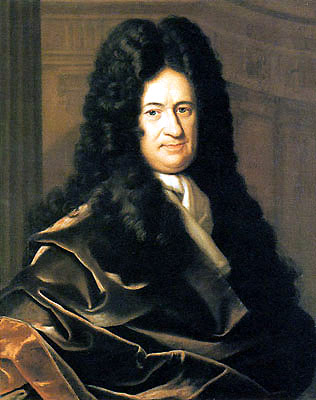
\includegraphics[width=0.384\textwidth]{leibniz.jpg}} 
		\subfigure[Isaac Newton]{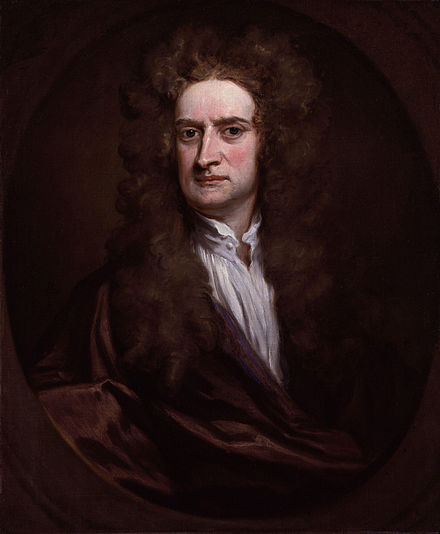
\includegraphics[width=0.4\textwidth]{newton.jpg}} 
		\caption{Die Entwickler der Differentialrechnung} 
	\end{figure} 
\end{frame}	

\begin{frame}{Differenzialrechnung - Newton}
	\begin{example}
		Beim freien, reibungsfreien Fall eines Regentropfens gibt die Wegfunktion
		\[
			s(t) = \frac{g}{2} t^{2} 
		\]
		den momentanen Ort in Abhängigkeit von der Fallzeit $t$ an. Wie groß ist die Geschwindigkeit in jedem Zeitpunkt $t$?
		
		Die mittlere Geschwindigkeit zwischen zwei Zeitpunkten $t_{1}$ und $t_{2}$ lässt sich einfach ausrechnen:
		\[
			\bar{v}_{t_{2}, t_{1}} = \frac{s(t_{2})-s(t_{1})}{t_{2}-t_{1}} = \frac{s(t_{1} + \Delta t) -s(t_{1})}{\Delta t}	
		\]
		mit $\Delta t := t_{2} - t_{1}$
	\end{example}
\end{frame}

\begin{frame}{Differenzialrechnung - Newton}
	\begin{example}
		Möchte man die Momentangeschwindigkeit bestimmen, muss man die Differenz $\Delta t := t_{2} - t_{1}$ beliebig klein machen. Da dann aber auch $\Delta s:=s(t_{1}+\Delta t) -  s(t_{1}) \to 0$ geht (weil der Weg ja stetig von der Zeit abhängt, der Tropfen macht im Flug ja keine Sprünge), muss man
		\[
			v(t):=\frac{ds(t)}{dt}:=\lim_{\Delta t \to 0} \frac{\Delta s(t)}{\Delta t}=\lim_{\Delta t \to 0} \frac{s(t+\Delta t)-s(t)}{\Delta t}
		\] 
		betrachten.
		Für das Weg-Zeit-Gesetz des Tropfens ist dann:
		\begin{align*}
			v(t)& =\lim_{\Delta t \to 0} \frac{\frac{g}{2}(t+\Delta t)^{2} - \frac{g}{2}t^{2}}{\Delta t} = \frac{g}{2} \lim_{\Delta t \to 0} \frac{t^{2} + 2t \Delta t + (\Delta t)^{2} -t^{2}}{\Delta t} \\
			& = \frac{g}{2} \lim_{\Delta t \to 0} \left( 2t + \Delta t \right) = \frac{g}{2} 2t = gt
		\end{align*}
	\end{example}
\end{frame}

\begin{frame}{Differenzialrechnung - Newton}
	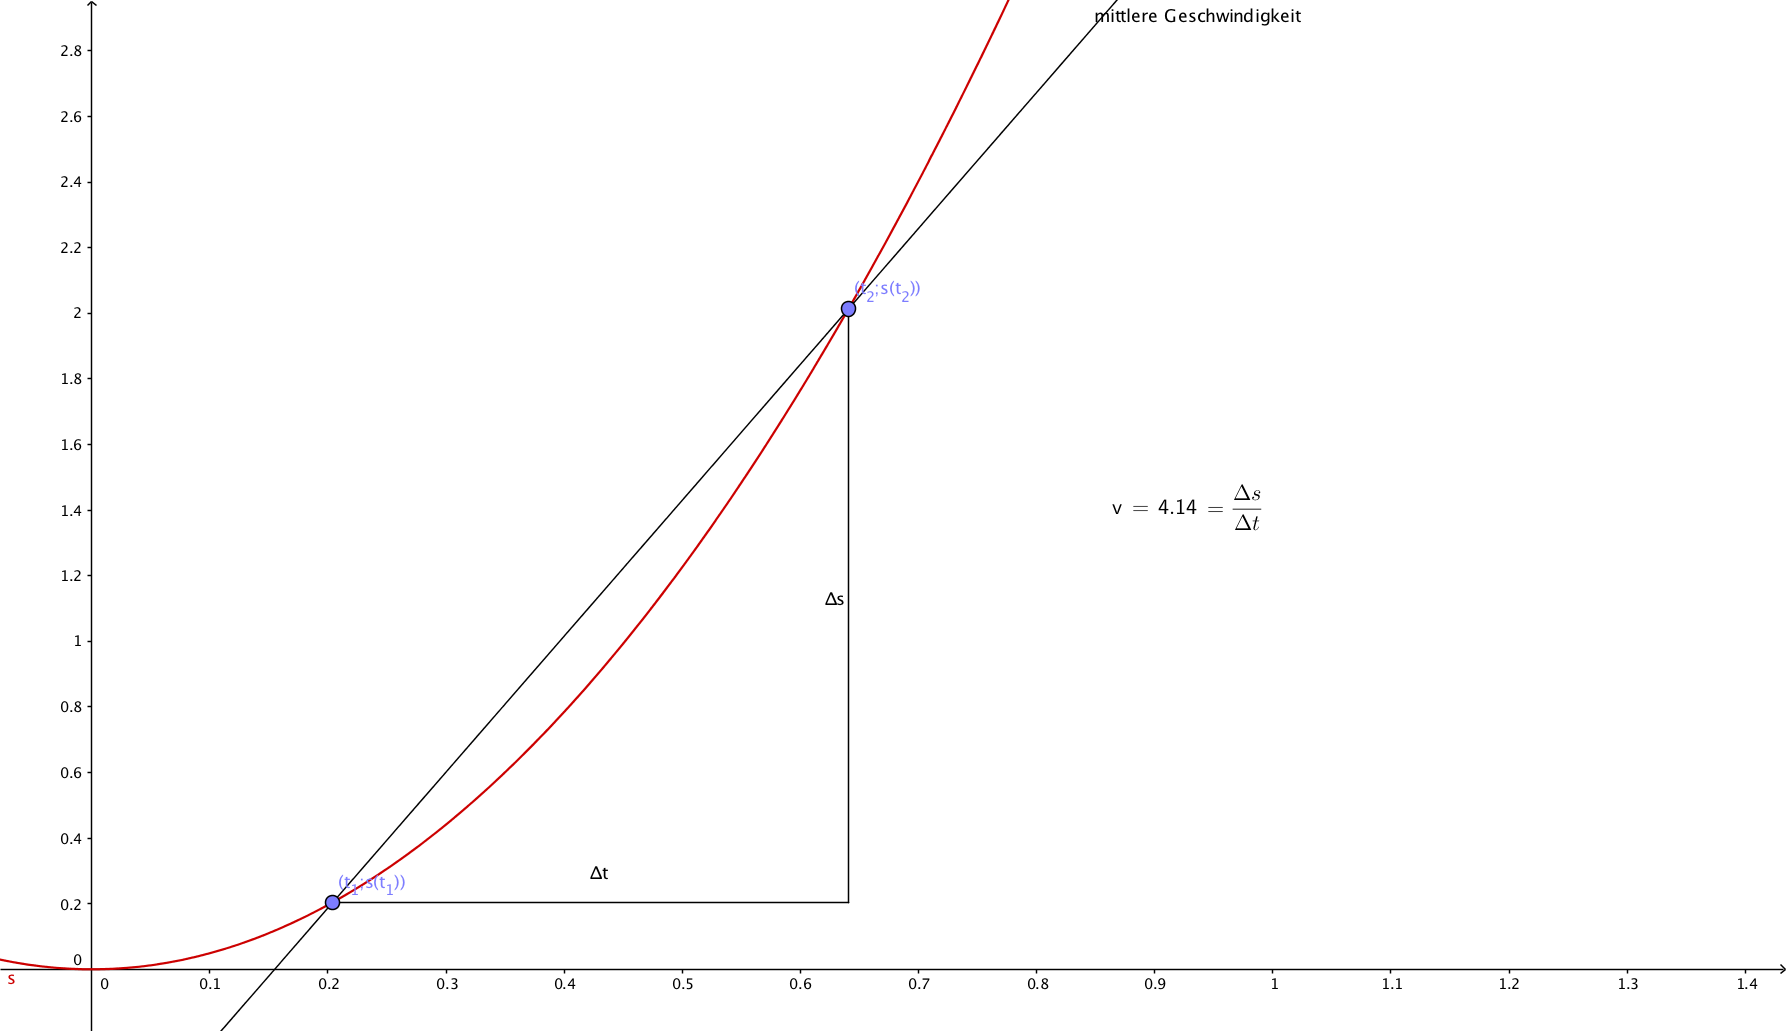
\includegraphics[width=14cm]{Geogebra/newton_geometrisch.png}
\end{frame}

\begin{frame}{Definition - Differenzialquotient}
	\begin{definition}{\small 	
		Existiert für eine (mindestens stetige) Funktion $y=f(x)$ an der Stelle $x_{0}$ der Grenzwert
		\[
			\lim_{\Delta x \to 0} \frac{\Delta y(x_{0})}{\Delta x} = \lim_{\Delta x \to 0} \frac{f(x_{0}+\Delta x)-f(x_{0})}{\Delta x} = \frac{dy(x_{0})}{dx} =: f' (x_{0}) =: y' (x_{0}) 
		\]
		so heißt dieser Grenzwert die \textbf{Ableitung von $f$} oder der \textbf{Differenzialquotient von $f$ an der Stelle $x_{0}$}.}
	
		Die Funktion heißt dann \textbf{differenzierbar an der Stelle $x_{0}$}.
		
		Wenn die Ableitung an allen Stellen $x \in D(f)$ existiert, kann man die Ableitung als eine Funktion $f'$ betrachten
		\[
			f'(x) := \lim_{\Delta x \to 0 } \frac{f(x+\Delta x)-f(x)}{\Delta x}  
		\] 
		und nennt diese Funktion $f'$ die \textbf{Ableitung von $f$}.
	\end{definition}
\end{frame}

\begin{frame}{Geometrische Deutung der Ableitung}
	\begin{bemerkung}
		Die erste Ableitung $f'(x_{0})$ gibt die Steigung der Tangente an den Graphen der Funktion $f$ an der Stelle $x_{0}$ an. Damit können also Aussagen gemacht werden über
		\begin{itemize}
			\item das Monotonieverhalten der Funktion $f$ und damit auch über
			\item evtl. Maxima und Minima der Funktion $f$.
		\end{itemize}
		Denn für den Differentialquotienten gilt ja:
		\[
			f'(x_{0}) = \lim_{x \to x_{0}} \frac{f(x)-f(x_{0})}{x-x_{0}} 
		\]
		und die rechte Seite ist 
		\begin{itemize}
			\item strikt positiv, wenn $f$ streng monoton wachsend
			\item positiv, wenn $f$ monoton wachsend
			\item strikt negativ, wenn $f$ streng monoton fallend bzw. 
			\item negativ, wenn $f$ monoton fallend ist.
	\end{itemize}
	\end{bemerkung}
\end{frame}

\begin{frame}{Beispiele für Ableitungen}
	\begin{example}
		Die \textbf{konstante Funktion} $f(x)=a$ ist überall differenzierbar und die Ableitung ist $f'(x) = 0$ für alle $x \in \mathbb{R}$. Denn
		\[
				\lim_{\Delta x \to 0} \frac{f(x+\Delta x) - f(x)}{\Delta x} = \lim_{\Delta x \to 0} \frac{a-a}{\Delta x} = \lim_{\Delta x \to 0} \frac{0}{\Delta x} = 0				
		\]
	\end{example}
	\begin{example}
		Die \textbf{lineare Funktion} $f(x)=mx+b$ mit $m,b \in \mathbb{R}$ ist überall differenzierbar und die Ableitung ist $f'(x) = m$ für alle $x \in \mathbb{R}$. Denn
		\begin{align*}
		\lim_{\Delta x \to 0} \frac{f(x+\Delta x) - f(x)}{\Delta x} & = \lim_{\Delta x \to 0} \frac{m(x+\Delta x)+b - (mx+b)}{\Delta x} \\ &= \lim_{\Delta x \to 0} \frac{m\Delta x}{\Delta x} = m				
		\end{align*}
	\end{example}
\end{frame}

\begin{frame}{Beispiele für Ableitungen}
	\begin{example}
		Die \textbf{quadratische Funktion} $f(x)=ax^{2}+bx+c$ mit $a,b,c \in \mathbb{R}$ ist überall differenzierbar und die Ableitung ist $f'(x) = 2ax+b$ für alle $x \in \mathbb{R}$. Denn
		\begin{align*}
		\lim_{\Delta x \to 0} & \frac{f(x+\Delta x) - f(x)}{\Delta x} \\ & = \lim_{\Delta x \to 0} \frac{a(x+\Delta x)^{2}+b(x+\Delta x) +c - (ax^{2}+bx+c)}{\Delta x} \\ &= \lim_{\Delta x \to 0} \frac{ax^{2} +2ax\Delta x +a(\Delta x)^{2} + bx +b \Delta x +c -ax^{2} - bx -c}{\Delta x} \\ &= \lim_{\Delta x \to 0  } \frac{2ax\Delta x + a(\Delta x)^{2} +b\Delta x}{\Delta x} = 2ax+b + \lim_{\Delta x \to 0} \frac{(a\Delta x)^{2}}{\Delta x}				
		\end{align*}
	\end{example}
\end{frame}

\begin{frame}{Beispiele für Ableitungen}
	\begin{example}
		Die \textbf{hyperbolische Funktion} $f(x)=\frac{1}{x}$ ist für alle $x\in D(f)=\mathbb{R}\setminus \{ 0 \}$ differenzierbar und die Ableitung ist $f'(x) = -\frac{1}{x^{2}}$ für alle $x \in D(f)$. Denn
		\begin{align*}
		\lim_{\Delta x \to 0} \frac{f(x+\Delta x) - f(x)}{\Delta x} & = \lim_{\Delta x \to 0} \frac{\frac{1}{x+\Delta x} - \frac{1}{x}}{\Delta x} \\ &= \lim_{\Delta x \to 0} \frac{\frac{x-(x+\Delta x)}{x(x+\Delta x)}}{\Delta x} \\ & = \lim_{\Delta x \to 0 } \frac{-\Delta x}{(\Delta x) x (x+\Delta x)} = -\frac{1}{x^{2}}			
		\end{align*}
	\end{example}	
\end{frame}

\begin{frame}{Ableitungen elementarer Funktionen}

{\LARGE $\begin{array}{cc}
	f(x)= x^{r} & f'(x)=r x^{r-1}  \\ 
	f(x)= \sqrt{x}& f'(x)=\frac{1}{2\sqrt{x}}  \\ 
	f(x)= \frac{1}{\sqrt{x}}& f'(x)= -\frac{1}{2\sqrt{x^{3}}}  \\ 
	f(x)= \log_{a} x & f'(x)=\frac{1}{x \ln a}  \\ 
	f(x)= a^{x}& f'(x)= a^{x} \ln a  \\ 
	f(x)= \sin x& f'(x)=\cos x \\ 
	f(x)= \cos x& f'(x)= -\sin x	  \\
\end{array} $
}
\end{frame}

\begin{frame}{Zweite und höhere Ableitungen}
	\begin{definition}
		Sofern man die Ableitung $f'$ einer Funktion $f$ wieder ableiten kann, so nennt man die Ableitung der Ableitungsfunktion $f'$ die zweite Ableitung der Funktion $f$ und bezeichnet sie mit $f''$.
		
		Eine Funktion $f$ heißt n-mal differenzierbar, wenn die n-te Ableitung existiert:
		\[
			\frac{d^{n}f(x)}{dx^{n}} = \frac{d}{dx}\frac{d^{n-1}f(x)}{dx^{n-1}} = f^{(n)}(x)
		\]
	\end{definition}
\end{frame}

\begin{frame}{Ableitungsregeln}
	\begin{theorem}
		Für zwei differenzierbare Funktion $f$ und $g$ gilt:
		\begin{itemize}
			\item Die Summe $f+g$ ist differenzierbar, also die Funktion $\left( f+g \right) (x) := f(x)+g(x)$ und $\left(f+g\right)'(x) = f'(x)+g'(x)$
			\item Die Differenz $f-g$ ist differenzierbar, also die Funktion $\left(f-g\right)(x) := f(x)-g(x)$ und $\left(f-g\right)'(x) = f'(x)-g'(x)$
			\item Die Funktion $c \cdot f$ mit einer Konstanten $c$ ist differenzierbar, also die Funktion $\left(c\cdot f\right)(x) := c\cdot f(x)$ und $\left(cf\right)'(x) = c\cdot f'(x)$				
			\item Die Funktion $f + c$ mit einer Konstanten $c$ ist differenzierbar, also die Funktion $f(x) + c$ und ihre Ableitung ist gleich $f'(x)$				
		\end{itemize}
	\end{theorem}
\end{frame}

\begin{frame}{Produktregel für die Ableitung}
	\begin{theorem}
		Das Produkt $h=f \cdot g$ zweier differenzierbarer Funktionen $f$ und $g$ ist differenzierbar und es gilt:
		\[
		h'(x)=\left( f\cdot g \right)' (x) = f'(x)\cdot g(x) + f(x)\cdot g'(x) 
		\]
	\end{theorem}
	\begin{proof}[Beweis]{
\tiny

 		\begin{align*}
		h'(x) & = \lim_{\Delta x \to 0} \frac{h(x+\Delta x) - h(x)}{\Delta x} \\
		& = \lim_{\Delta x \to 0} \frac{f(x+\Delta x)\cdot g(x+\Delta x) - f(x)\cdot g(x)}{\Delta x} \\
		& = \lim_{\Delta x \to 0} \frac{f(x+\Delta x)\cdot g(x+\Delta x) - f(x)\cdot g(x)}{\Delta x} \\
		& = \lim_{\Delta x \to 0} \frac{f(x+\Delta x)\cdot g(x+\Delta x) - f(x)\cdot g(x+\Delta x) + f(x)\cdot g(x+\Delta x)- f(x)\cdot g(x)}{\Delta x}  \\			
		& = \lim_{\Delta x \to 0} \frac{\left( f(x+\Delta x) - f(x)\right)\cdot g(x+\Delta x) + f(x)\cdot \left( g(x+\Delta x )- \cdot g(x)\right) }{\Delta x}  \\			
		& = f'(x)\cdot g(x) + f(x)\cdot g'(x)
		\end{align*}}
	\end{proof}
\end{frame}

\begin{frame}{Quotientenregel für die Ableitung}

{\small	\begin{theorem}
		Der Quotient $h=\frac{f}{g}$ zweier differenzierbarer Funktionen $f$ und $g$ ist differenzierbar an allen Stellen, an denen $g(x)\neq 0$ ist und es gilt:
		\[
		h'(x)=\left( \frac{f}{g} \right)' (x) = \frac{f'(x)\cdot g(x) - f(x)\cdot g'(x)}{g^{2}(x)} 
		\]
	\end{theorem}
}	\begin{proof}[Beweis]{\tiny
		\begin{align*}
		h'(x) & = \lim_{\Delta x \to 0 } \frac{1}{\Delta x} \left( \frac{f(x+\Delta x)}{g(x+\Delta x)} - \frac{f(x)}{g(x)} \right) \\
		&= \lim_{\Delta x \to 0 } \frac{1}{\Delta x} \left( \frac{f(x+\Delta x) g(x)}{g(x+\Delta x) g(x)} - \frac{f(x)g(x+\Delta x)}{g(x)g(x+\Delta x)} \right) \\
		&= \lim_{\Delta x \to 0 } \frac{1}{g(x+\Delta x) g(x)} \left( \frac{f(x+\Delta x) g(x)- f(x)g(x+\Delta x)}{\Delta x} \right) \\
		&= \lim_{\Delta x \to 0 } \frac{1}{g(x+\Delta x) g(x)} \left( \frac{f(x+\Delta x) g(x)-f(x)g(x)+f(x)g(x)- f(x)g(x+\Delta x)}{\Delta x} \right) \\
		&= \lim_{\Delta x \to 0 } \frac{1}{g(x+\Delta x) g(x)} \left(  \frac{\left(f(x+\Delta x) -f(x)\right) g(x)-f(x)\left( g(x+\Delta x) -g(x)\right) }{\Delta x} \right) 				
\end{align*}}
	\end{proof}
\end{frame}

\begin{frame}{Kettenregel - Motivation}
	\begin{bemerkung}
		Bisher wurden Ableitungen elementarer Funktionen sowie Summen, Produkte und Quotienten behandelt.
		
		Damit sind aber Ableitung von Funktionen wie z.B. 
		\[
			e^{(4x^{2}-3x+2)} \qquad \text{ oder }\qquad \sin (3x+\alpha)
		\]
		nicht möglich.
		
		Diese Funktionen sind \textbf{verkettete Funktionen} $h(x):=f(g(x))$, bei denen man zuerst die \textbf{innere Funktion} $g$ auf $x$ anwendet und dann das Ergebnis $g(x)$ in die \textbf{äußere Funktion} $f$ einsetzt.
		
		In den Beispielen oben ist $g(x)=4x^{2}-3x+2$ und $f(g)=e^{g}$ bzw. $g(x)=3x+\alpha$ und $f(g)=\sin (g)$.
	\end{bemerkung}
\end{frame}

\begin{frame}{Kettenregel für die Ableitung\footnote{Ableitung der mittelbaren Funktion}}
	\begin{theorem}
		Für zwei auf ihrem jeweiligen Definitionsbereich differenzierbare Funktionen $f$ und $g$ mit $W(g) \subset D(f)$ (d.h. man kann die $y$-Werte von $g$ in $f$ einsetzen.) sei $h$ die Verkettung der beiden Funktionen, also
		\[
			h(x):= f(g(x)) \qquad \forall x \in D(f)
		\]
		Dann gilt für die Ableitung von $h$:
		\[
			h'(x)=f'(g(x)) \cdot g'(x) \qquad \forall x \in D(f)
		\]
		Man nennt $f'(g(x))$ die \textbf{äußere Ableitung} und $g'(x)$ \textbf{die innere Ableitung}.
	\end{theorem}
\end{frame}

\begin{frame}{Kettenregel - sowas wie ein Beweis}

{\small 	\begin{bemerkung}
				Betrachtet man die äußere Funktion als Funktion von $g$, so ist
				\[
				\frac{df}{dg} = \lim_{\Delta g \to 0} \frac{f(g+\Delta g)-f(g)}{\Delta g} = \lim_{\Delta g \to 0} \frac{\Delta f}{\Delta g}
				\]	
				und entsprechend ist für die innere Funktion $g$ als Funktion von $x$
				\[
				\frac{dg}{dx} = \lim_{\Delta x \to 0} \frac{g(x+\Delta x)-g(x)}{\Delta x} = \lim_{\Delta x \to 0} \frac{\Delta g}{\Delta x}
				\]	
		Für die verkettete Funktion $h(x)=f(g(x))$ wäre der Differenzialquotient
		\begin{align*}
			\frac{dh}{dx} & = \lim_{\Delta x \to 0} \frac{h(x+\Delta x)-h(x)}{\Delta x} = \lim_{\Delta x \to 0} \frac{\Delta h}{\Delta x} \\
			& = \lim_{\Delta x \to 0} \frac{\Delta (f(g(x)))}{\Delta x} = \lim_{\Delta x \to 0 } \left( \frac{\Delta f(g(x))}{\Delta g(x)} \frac{\Delta g(x)}{\Delta x} \right)  \\
			& = \lim_{\Delta g \to 0 } \frac{\Delta f(g)}{\Delta g} \lim_{\Delta x \to 0 } \frac{\Delta g(x)}{\Delta x} = f'(g(x))\cdot g'(x)
		\end{align*}		
		\end{bemerkung}
}\end{frame}

\begin{frame}{Ableitung der Umkehrfunktion}
	\begin{theorem}
		Für die Umkehrfunktion $f^{-1}$ einer differenzierbaren Funktion $f$ gilt:
		\[
			\left(f^{-1}\right)' (x) = \frac{1}{f'(f^{-1}(x))}
		\]
	\end{theorem}
{\small	\begin{bemerkung}
		Man kann sich das so merken:
		\begin{align*}
		& f\left(f^{-1}(x)\right) & = x \\ & \Rightarrow \frac{d}{dx} f\left(f^{-1}(x)\right) & = \frac{d}{dx} x = 1 \\  & \Rightarrow f'\left( f^{-1}(x) \right)  \left( f^{-1} \right)'(x) & = 1 \\ 
		& \Rightarrow \left( f^{-1} \right)'(x) & = \frac{1}{f'(f^{-1}(x))}
		\end{align*}
	\end{bemerkung}}
\end{frame}

\begin{frame}{Regel von l'Hospital\footnote{Guillaume François Antoine, Marquis de L’Hospital hat die Regel nicht selbst entdeckt, sondern von Johann Bernoulli gekauft!}}

{\footnotesize	\begin{bemerkung}
		Die Regel von l'Hospital dient zur Berechnung von Grenzwerten $\lim_{x \to x_{0}}\frac{f(x)}{g(x)}$, bei denen unbestimmte Ausdrücke der Form
		\[
		\frac{\infty}{\infty} \quad \frac{0}{0} \quad 0\cdot \infty \quad 0^{0} \quad 1^{\infty} \quad \infty - \infty
		\]
	\end{bemerkung}
	\begin{theorem}
		Sind $f$ und $g$ in einem Intervall um $x_{0}$ differenzierbare Funktionen und $g(x)\neq 0$ in einer Umgebung von $x_{0}$, aber entweder 
		\begin{itemize}
			\item 
		$\lim_{x \to x_{0}} g(x) = 0$ und $\lim_{x \to x_{0}} f(x) = 0$ oder
		\item $\lim_{x \to x_{0}} g(x) = \infty$ und $\lim_{x \to x_{0}} f(x) = \infty$
	\end{itemize} 
	wobei der Grenzwert
	\[
		\lim_{x \to x_{0}} \frac{f'(x)}{g'(x)}
	\]
	existiert, so gilt:
	\[
		\lim_{x \to x_{0}} \frac{f(x)}{g(x)} = \lim_{x \to x_{0}} \frac{f'(x)}{g'(x)}
	\]
	\end{theorem}}
\end{frame}

\begin{frame}{Regel von l'Hospital - sowas wie ein Beweis}
	\begin{bemerkung}
		Für den Fall $f(x_{0})=g(x_{0}) = 0$ kann man das anschaulich so erklären:
		\[
			\lim_{x \to x_{0}} \frac{f(x)}{g(x)} = \lim_{x \to x_{0}} \frac{f(x)-f(x_{0})}{g(x)-g(x_{0})} = \lim_{x \to x_{0}} \frac{\frac{f(x)-f(x_{0})}{x-x_{0}}}{\frac{g(x)-g(x_{0})}{x-x_{0}}} = \frac{f'(x_{0})}{g'(x_{0})}
		\]
		Im ersten Schritt hat man hier im Zähler und im Nenner jeweils eine 0 hinzugefügt, im zweiten Schritt mit $x-x_{0}$ erweitert und dann die Definition der Ableitung benutzt.
		
		Die verbleibenden Grenzwertfälle müssen durch Äquivalenzumformungen auf diese beiden Fälle zurückgeführt werden.
	\end{bemerkung}
\end{frame}

\begin{frame}{Geometrische Deutung der 1. Ableitung}
	\begin{bemerkung}
		Die erste Ableitung $f'$ einer Funktion $f$ gibt die Steigung der Tangente an den Graphen der Funktion f an. Daher können mit Hilfe der 1. Ableitung Aussagen über das Monotonie-Verhalten der Funktion $f$ gemacht werden:
		\begin{itemize}
			\item Falls $f'(x_{0})>0$, so ist die Funktion in einer Umgebung von $x_{0}$ streng monoton wachsend.
			\item Falls $f'(x_{0})<0$, so ist die Funktion in einer Umgebung von $x_{0}$ streng monoton fallend.	
		\end{itemize}  
	\end{bemerkung}
\end{frame}

\begin{frame}{Relative/lokale Extrema - Definition}
	\begin{definition}
		Die Funktion $f$ hat an der Stelle $x_{0}$ ein \textbf{relatives/lokales Maximum}, wenn für alle $x$ in einer Umgebung von $x_{0}$ gilt: 
		\[
		f(x_{0})>f(x)
		\]
		
		Die Funktion $f$ hat an der Stelle $x_{0}$ ein \textbf{relatives/lokales Minimum}, wenn für alle $x$ in einer Umgebung von $x_{0}$ gilt: 
		\[
		f(x_{0})<f(x)
		\]
		
		In beiden Fällen spricht man von einem \textbf{relativen/lokalen Extremum}.
	\end{definition}
\end{frame}
\begin{frame}{Lokale Extrema - Notwendige Bedingung}
	\begin{theorem}[Fermat]
		Falls eine differenzierbare Funktion $f$ im Punkt $x_{0}$ ein relatives Extremum hat, so gilt dort:
		\[
			f'(x_{0}) = 0
		\]
		Die Bedingung ist \textbf{notwendig}, aber \textbf{nicht hinreichend}, denn es gibt Funktionen mit waagerechter Tangente, die dort kein Extremum haben.
	\end{theorem}
\end{frame}

\begin{frame}{Zwischenwertsatz - Satz von Rolle - Mittelwertsatz}

{\footnotesize	\begin{theorem}[Zwischenwertsatz]
		Für eine stetige Funktion $f$ mit $f(a) \leq f(b)$ und $a<b$ gilt:
		\[
		\text{Für alle }y_{0} \text{ mit } f(a)\leq y_{0} \leq f(b) \text{ gibt es ein } x_{0} \text{ mit } a \leq x_{0} \leq b \text{ und } f(x_{0})=y_{0}
		\]
	\end{theorem}
	\begin{theorem}[Rolle]
		Für jede differenzierbare Funktion $f$ mit $f(a)=f(b)$ gibt es eine Stelle $x_{0}$ mit $f'(x_{0}) = 0$.
	\end{theorem}
	\begin{theorem}[Mittelwertsatz]
		Ist eine Funktion $f$ im Intervall $[a, b]$ stetig und in $]a, b[$ differenzierbar, dann gibt es eine Stelle $x_{0}$ mit $a < x_{0} < b$ und 
		\[
			f'(x_{0}) = \frac{f(b)-f(a)}{b-a}
		\]
	\end{theorem}
}
\end{frame}

\begin{frame}{Extrema - notwendige und hinreichende Bedingung}
	\begin{theorem}
		Eine differenzierbare Funktion $f$ besitzt an der Stelle $x_{0}$ ein relatives/lokales Extremum, wenn gilt:
		\[
			f'(x_{0}) = 0 \qquad \text{und}\qquad f^{(n)}(x_{0}) \neq 0 \text{ für ein gerades } n. \footnote{z.B. und meistens $n=2$} 
		\]
		Genauer ist:
		\begin{itemize}
			\item an der Stelle $x_{0}$ ein \textbf{relatives Maximum}, falls $f'(x_{0})=0$ und $f^{(n)}(x_{0})<0$ für ein gerades $n$.
			\item an der Stelle $x_{0}$ ein \textbf{relatives Minimum}, falls $f'(x_{0})=0$ und $f^{(n)}(x_{0})>0$ für ein gerades $n$.
		\end{itemize}
	\end{theorem}
\end{frame}

\begin{frame}{Randextrema}
\begin{bemerkung}
	Bei Funktionen, deren Definitionsbereich eingeschränkt (z.B. auf ein Intervall) ist, kann es sein, dass Extrema an den Rändern des Definitionsbereiches angenommen werden, obwohl dort die (dann meist nur einseitig definierte Ableitung) nicht null ist.
	
	Beispiel: $f(x)=\sqrt{1-x^{2}}$
	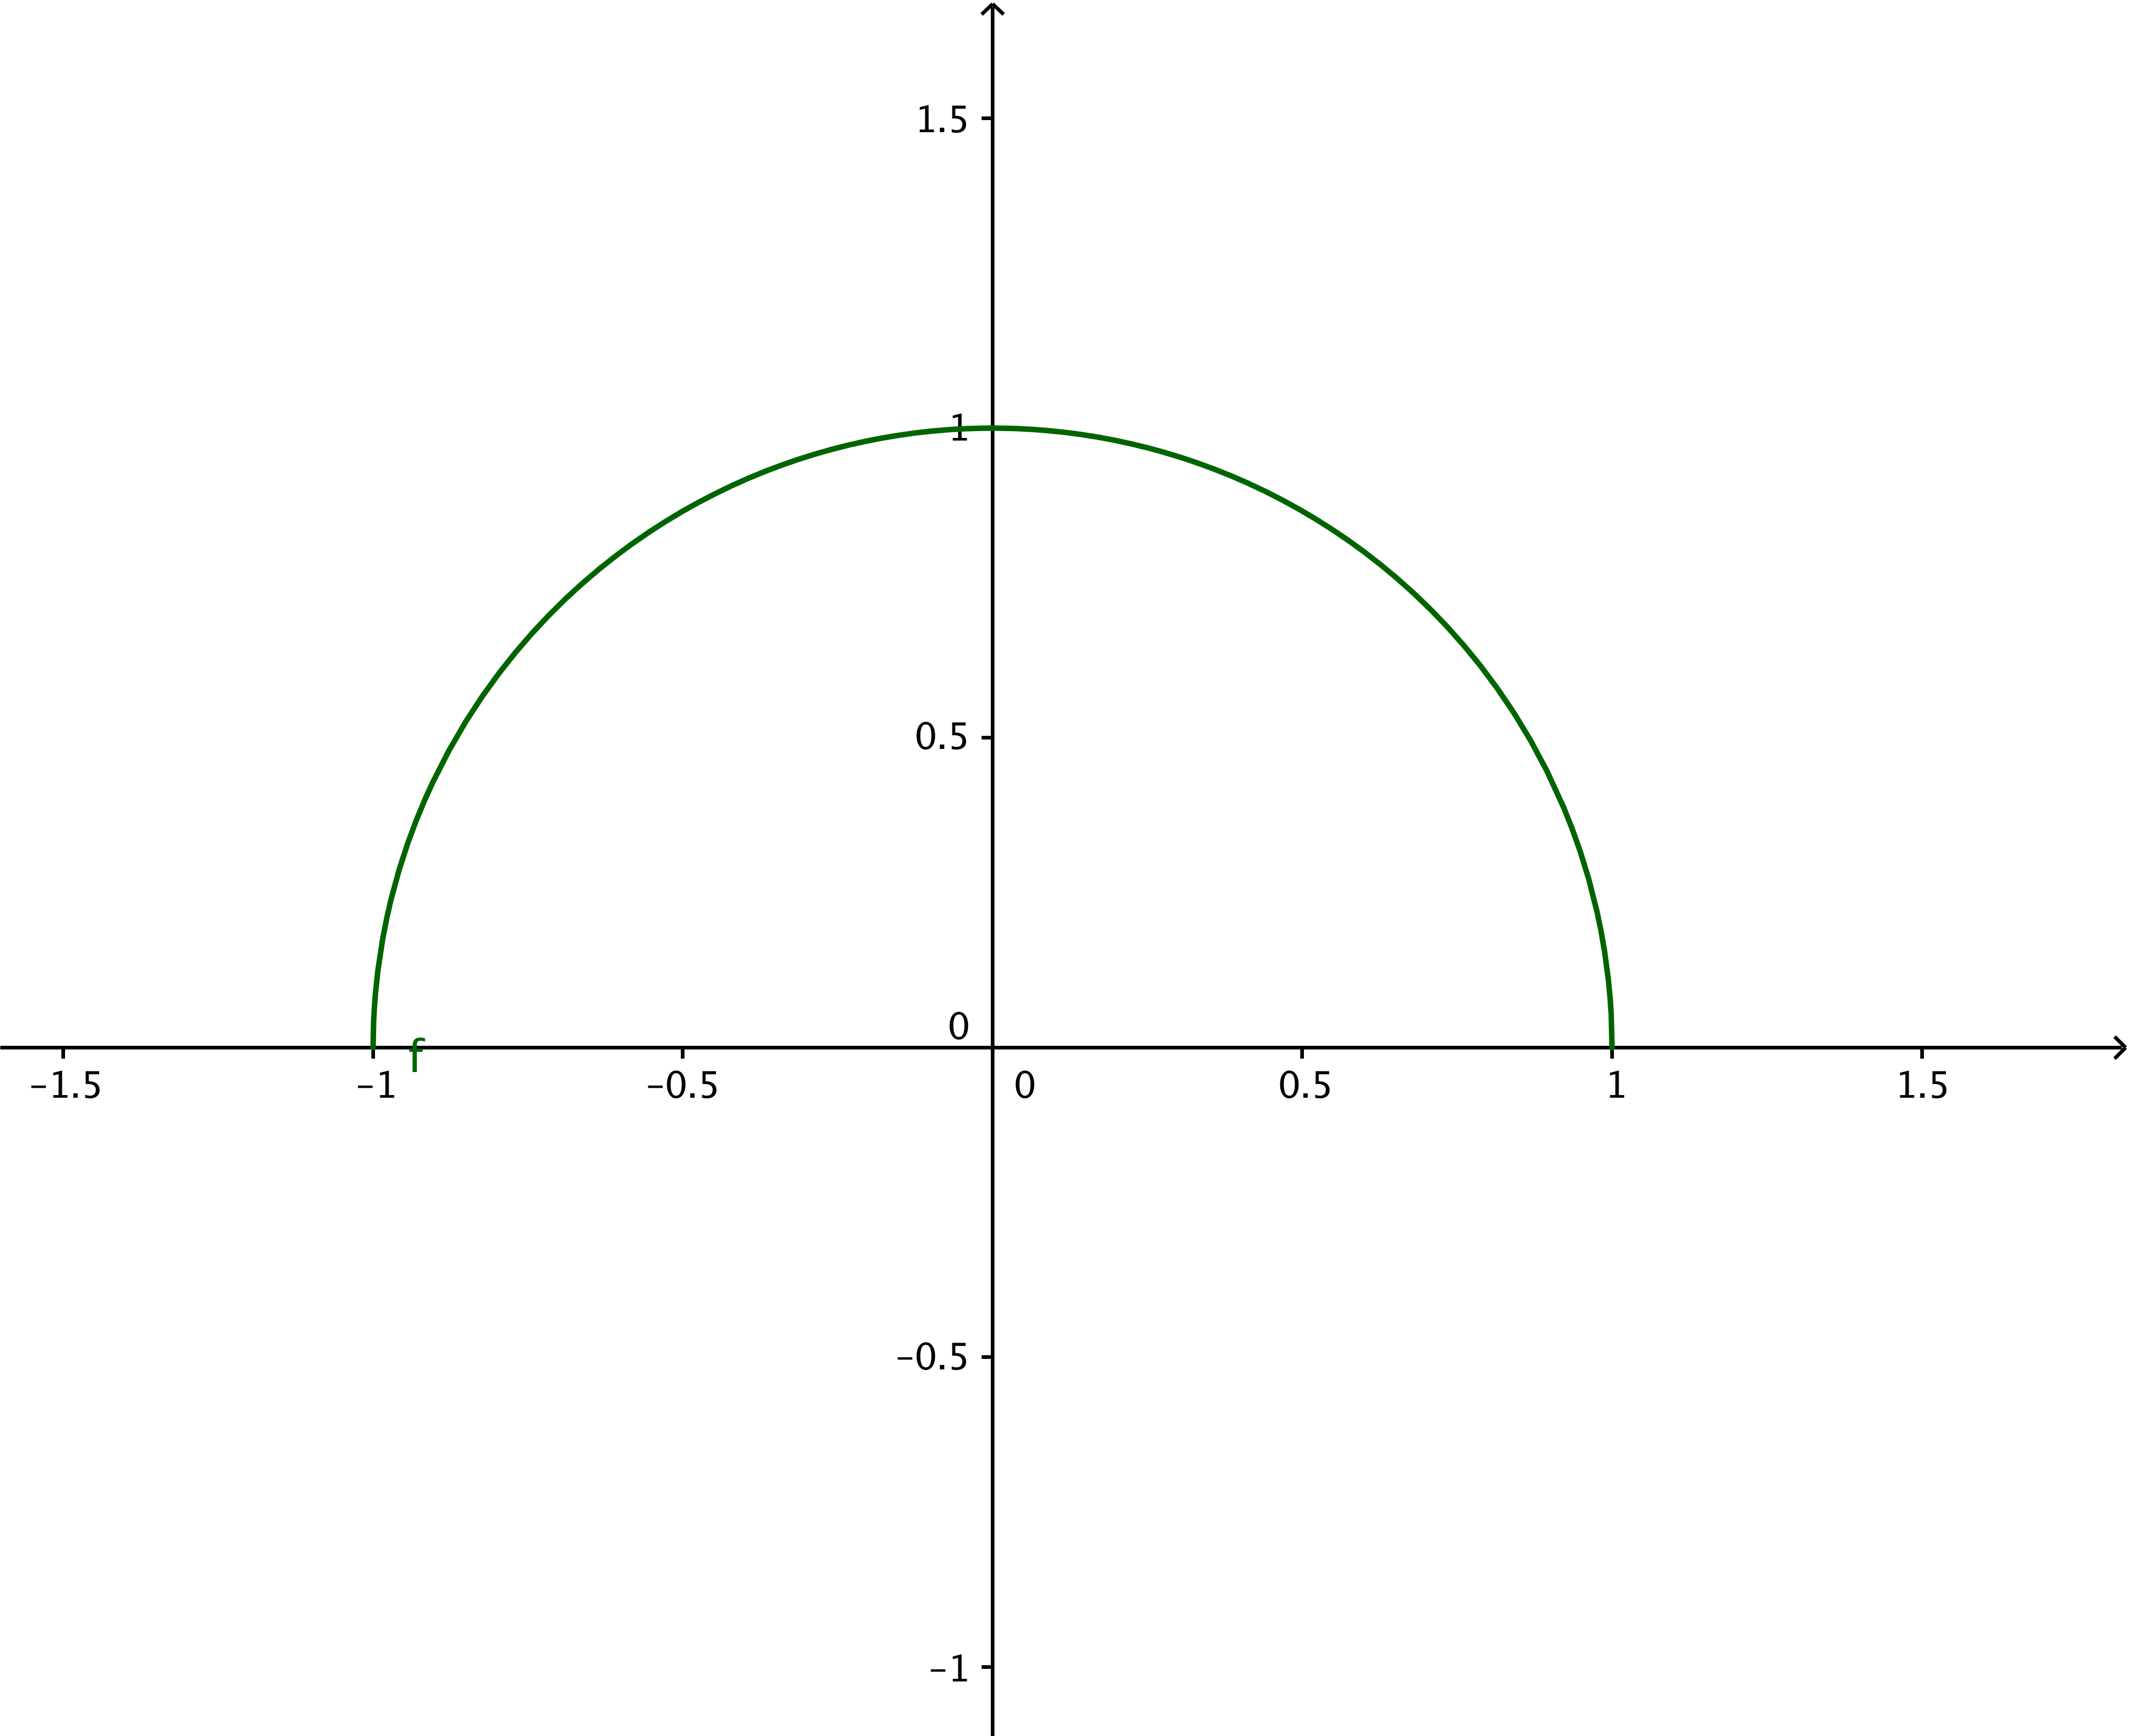
\includegraphics[width=9cm]{halbkreis}
\end{bemerkung}	
\end{frame}

\begin{frame}{Geometrische Deutung der 2. Ableitung}
\begin{bemerkung}
	Die erste Ableitung einer Funktion $f$ gibt deren Steigung an jeder Stelle an. Die Veränderung dieser Steigung gibt die zweite Ableitung (als Ableitung der 1. Ableitung) an.
	
	Wenn die Steigung einer Funktion zunimmt, also die 2. Ableitung positiv ist, ist die Funktion linksgekrümmt.
	
	Wenn die Steigung einer Funktion abnimmt, also die 2. Ableitung negativ ist, ist die Funktion rechtsgekrümmt.
\end{bemerkung}
\begin{definition}
	Für eine zweimal differenzierbare Funktion $f$ gilt:
	\begin{itemize}
		\item $f$ heißt streng \textbf{linksgekrümmt} oder \textbf{streng konvex} im Punkt $x_{0}$, wenn $f''(x_{0})>0$ ist.
		\item $f$ heißt streng \textbf{rechtsgekrümmt} oder \textbf{streng konkav} im Punkt $x_{0}$, wenn $f''(x_{0})<0$ ist.
	\end{itemize} 
\end{definition}
\end{frame}

\begin{frame}{Wende- und Sattelpunkte}
\begin{definition}
	Die Stellen, an denen eine Funktion ihr Krümmungsverhalten von rechts- auf linksgekrümmt (oder umgekehrt) ändert, heißen \textbf{Wendepunkte}.
	
	Wenn zudem die Tangente an einem Wendepunkt waagerecht ist, nennt man den Wendepunkt einen \textbf{Sattelpunkt}. 	
\end{definition}
\begin{theorem}
	Eine dreimal differenzierbare Funktion $f$ besitzt an der Stelle $x_{0}$ einen Wendepunkt genau dann, wenn 
	\[
		f''(x_{0}) = 0 \quad \text{und} \quad f'''(x_{0})\neq 0
	\]
	ist.
	Wenn zudem $f'(x_{0}) = 0$ ist, so hat die Funktion an der Stelle $x_{0}$ einen Sattelpunkt.
\end{theorem}
\end{frame}
\begin{frame}{Krümmungseigenschaften}
\begin{bemerkung}
	Die dritte Ableitung $f'''$ einer Funktion $f$ gibt dabei offenbar an, in welche Richtung der Krümmungswechsel stattfindet\footnote{natürlich nur, wenn $f''(x_{0})=0$ ist}:
	\begin{itemize}
		\item Falls $f'''(x_{0})>0$ ist, so wechselt die Krümmung von Rechts- auf Linkskrümmung.
		\item Falls $f'''(x_{0})<0$ ist, so wechselt die Krümmung von Links- auf Rechtskrümmung.
	\end{itemize}
\end{bemerkung}
\end{frame}

\begin{frame}{Kurvendiskussion}
	\begin{bemerkung}
		Alle bisherigen Hilfmittel zur Untersuchung einer Funktion lassen sich zusammenfassen in einer \textbf{Kurvendiskussion}. Diese beinhaltet:
		\begin{enumerate}
			\item Bestimmung der Definitionsmenge und der Wertemenge
			\item Untersuchung auf Symmetrie und Periodizität
			\item Bestimmung von Nullstellen, Verhalten an Definitionslücken, Polstellen, Verhalten für $x \to \pm \infty$
			\item Untersuchung auf Stetigkeit und Differenzierbarkeit
			\item Bestimmung der Extrema und Wendepunkte
			\item Graph der Funktion
		\end{enumerate}
	\end{bemerkung}
\end{frame}

\begin{frame}{Extremwertaufgaben}
	\begin{example}
		Aus einem rechteckigen Blech mit den Seitenlängen $a$ und $b$ ist nach dem Herausschneiden von quadratischen Flächen der Kantenlänge $x$ an den Ecken ein oben offener Kasten mit möglichst großem Volumen zu formen.
		
		Für das Volumen gilt:
		\[
		V(x)=\left( a-2x \right) \left( b-2x \right) x = 4x^{3} -2(a+b)x^{2} +abx 
		\]
		
		Dessen Maximum könnte an den Stellen sein, wo die Ableitung verschwindet:
		
		\[
		V'(x)=12x^{2} -4 (a+b)x + ab \overset{!}{=} 0 \]
		also an den Stellen
		\[
		x_{1,2} = \frac{1}{6} \left( a+b\pm \sqrt{a^2+b^2-ab} \right)
		\]
	\end{example}
\end{frame}

\begin{frame}{Extremwertaufgaben}
	\begin{example}
		Zur Überprüfung, ob es sich wirklich an beiden Stellen um Maxima handelt, setzt man diese Stellen in die zweite Ableitung
		\[
			V''(x)=24x-4(a+b)
		\]
		ein:
		\[
		V''(x_{1})= 24 x_{1} -4(a+b) = 4\sqrt{a^2+b^2-ab} > 0
		\]
		und 
		\[
		V''(x_{2})= 24 x_{2} -4(a+b) = - 4\sqrt{a^2+b^2-ab} < 0		
		\]
		Also ist nur an der Stelle $x_{2}$ die Volumenfunktion $V(x)$ rechtsgekrümmt mit waagerechter Tangente und entsprechend handelt es sich bei dieser Stelle $x_{2}$ und das lokale Maximum. Das maximale Volumen ist dann $V(x_{2})$.
	\end{example}
\end{frame} 